\chapter{Spectrum Analyzer}
\label{SpectrumAnalyzerAppendix}

In this Appendix, we discuss the Fabry-Perot spectrum analyzer that we built to analyze this system. 


\section{Spectrum analyzer design}
One of the mirrors is mounted on a Thorlabs kinematic piezo mount and attached to a piezo driver designed specifically for spectrum analyzers.

The cavity is designed to be nearly semiconfocal.%\footnote{I used to think that this was because the transverse modes of a semiconfocal cavity overlap. However, it seems that a concentric cavity would be more likely to have this property. Oh wait. I get it. The semiconfocal cavity has all its transverse modes very small.} 
This is because a semiconfocal configuration is one of several in which many modes are degenerate, such that liht coupling to different transverse modes come into resonnance at the same frequency. This makes it possible to get very sharp, clear features without having to carefully couple to one specific transverse mode of the cavity. 

%\footnote{How do I know whether I'm semiconfocal for all practical purposes? I mean, somehow lower finesse should make me less sensitive to small variations in the cavity length. Furthermore, are there models where the errors never really go away? You know? I guess I mean where it doesn't just become part of the noise. I suppose chaos is one example of this--where arbitrarily high precision is needed to predict even the macroscopic behavior of the system. Is any aspect of this system chaotic?}

\section{Free spectral range basics}
The Free Spectral Range (FSR) of the cavity is defined as the difference in frequency between adjacent resonant longitudinal modes of the cavity. It always works out to be $c/2L$. 
It is easy to condsider the example of a one-dimensional cavity with just one transverse mode. If we suppose that we have some wavelength $\lambda$ that is resonant with our cavity, then the resonant condition would be that 
\begin{equation}
m\lambda=2L
\end{equation}
where $m$ is an integer and $L$ is the cavity length (center to center distance between the surfaces of the cavity mirrors). In other words, we require that for a mode to be resonant with our cavity, the total optical path length of a trip around the cavity (in this case, twice the cavity length) must be divisible by the wavelength of the light. We can find other wavelengths of light that satisfy the resonance condition. So, for example, we might be able to find some wavelength $\lambda'$ that satisifes
\begin{equation}
(m+1)\lambda'=2L
\end{equation}

The free spectral range would just be the difference in frequencies corresponding to $\lambda$ and $\lambda'$. Using $\lambda = c/f$, we see that 
\begin{equation}
m\lambda= 2L \rightarrow \frac{mc}{f}=2L
\end{equation}
which we can solve for $f$ to find 
\begin{align}
f-f'&= \frac{(m+1)c}{2L}-\frac{m c}{2L}\\
&= \frac{c}{2L}
\end{align}

where $f'$ and $f'$ are the frequencies associated with $\lambda$ and $\lambda'$ respectively. 

\section{Free spectral range for real cavities}
In general, there will be more than one transverse mode. The free spectral range remains $c/2L$. However, between any two peaks corresponding to one transverse mode, there will be other resonant peaks corresponding to other transverse modes. Thus, there will be resonances of our cavity spaced closer than the free spectral range. One could, in principle, couple to just a single transverse mode by carefully coupling the beam to the cavity.

However, in our system this is not necessary. We use a semiconfocal (hemiconfocal), which has the convenient property that the various transverse modes line up in such a way that they fall into four distinct, evenly-spaced groups. Therefore, if we couple to many transverse modes of the cavity, we expect that our effective free spectral range will be $c/8L$.

%\footnote{Look, I was very confused about the factor of 8 for a long time. I now realize that I was simply misinterpreting the normal ray transfer diagram I had in my mind of a confocal cavity. Also, I was not very clear on why semiconfocal was the one where different transverse modes overlap. Since I've found the answers, I figured I might as well put them here.} 
\section{Derivation of free spectral range for hemiconfocal cavities}
\begin{figure}
\centerline{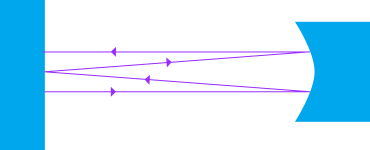
\includegraphics[height=3cm]{spectrum_analyzer_path.png}}
\caption[Spectrum analyzer ray path illustration]{\label{completePath}Illustration of the optical path that makes a complete trip around the semiconfocal cavity. Note that the ray traverses the entire length of the path four times before doubling back on itself. It traverses the path 8 times before ending up in the same place again. This diagram similar to one found on page 277 of Ref.\ \cite{lasersMilonniEberly}. Here, we assume that the ray travels nearly parallel to the central axis of the cavity so that the length of each leg is well-approximated by the length of the cavity, $L$.}
\end{figure}

This can be illustrated with a simple ray-tracing argument. 
In order for the cavity to be resonant with our light, the full optical path of the light must be an integer number of wavelengths. The resonance condition is 
\begin{equation}
n \lambda = d
\end{equation}
where $n$ is an integer, $\lambda$ is the wavelength and $d$ is the length of the optical path in the cavity. 
For a semiconfocal cavity, we can convince ourselves visually (see Fig.\,\ref{completePath}) that a ray parallel to the optical axis would traverse the entire length of the cavity 8 times before finally getting back to its starting point. Thus, we expect that $d\approx 8L$.
We therefore expect that modes in the cavity will have resonant frequencies spaced by $c/8L$. 


\section{Using the paraxial wave equation}

A more rigorous treatment of this can be done by solving the paraxial wave equation. This model will also allow us to model the exact behavior of our real life cavity (note that in the real cavity, we look at just a handful of wavelengths but we scan the cavity length).

\subsection{Review of paraxial wave equation}

We first examine the equation describing the electric field for different modes of the cavity. This can be derived directly from Maxwell's equations using the paraxial approximation (see, e.g., Refs.\ \cite{lasersMilonniEberly} and \cite{bergeson_amo_notes} for a complete discussion of this). The argument in brief is basically this: 

\begin{itemize}
\item Assume that the three-dimensional electric field can be represented by a scalar quantity $E(\mathbf{r},t)$
\item Recall Maxwell's equations with no nearby charges or currents give rise to the wave equation $\nabla^2E(\mathbf{r},t)-\frac{1}{c^2} \frac{\partial^2}{\partial t^2} E(\mathbf{r,t})=0$
\item Assume solution takes the form $E(\mathbf{r},t) = \mathcal{E}_0(\mathbf{r}) \exp(i(kz-\omega t))$ and plug this into the wave equation above. 
\item Make the paraxial approximation: Assume that $\lambda \left|\frac{\partial \mathcal{E}}{\partial z} \right| \ll |\mathcal{E}_0|$ and $\lambda \left| \frac{\partial^2\mathcal{E}_0}{\partial z^2}\right| \ll \left| \frac{\partial \mathcal{E}_0}{\partial z}\right|$. In other words, we assume that the wiggling
%\footnote{I think this word is so funny, but I might change it} 
is mostly happening along the $z$ direction. 
\end{itemize}

This leads to the paraxial wave equation: 
\begin{equation}
\left(\frac{\partial^2}{\partial x^2}+\frac{\partial^2}{\partial y^2}+2ik\frac{\partial}{\partial z}\right) \mathcal{E}_0(\mathbf{r})=0 \label{final_paraxial_wave_eqn}
\end{equation}

The solutions to Eq.\ \ref{final_paraxial_wave_eqn} can be shown to be of the form:

\begin{align} \label{solutionToParaxial}
\mathcal{E}_{mn}(x,y,z)=&\frac{Aw_o}{w(z)}H_m\left[\sqrt{2}\frac{x}{w(z)}\right]H_n\left[\sqrt{2}\frac{x}{w(z)}\right] \\
&\times \exp(i(kz-(m+n+1)\tan^{-1}(z/z_0)\\
&\times \exp(ik(x^2+y^2)/2R(z)) \exp(-(x^2+y^2)/w^2(z))
\end{align}

Here, $\mathcal{E}$ is the magnitude of the electric field. $H_m$ and $H_n$ are the (physicists') Hermite polynomials of degree $m$ and $n$\footnote{If we ever were to need a real solution to the equation, we could find one by simply taking: $\mathcal{E}+\mathcal{E}*$.}. $R(z)$,$z_0$,$w_z$ and $w_0$ are defined in the same way that they are for a Gaussian mode:

\begin{align}
w(z)&=w_0 \sqrt{1+\frac{z^2}{z_0^2}} \\
R(z)&=z+\frac{z_0^2}{z}\\
z_0&=\frac{\pi w_0^2}{\lambda }
\end{align}

%\footnote{I'm not sure why this works when we neglect polarization. It seems like you might get accidentally a factor of 2 or something extra based on the polarization diagram that Milloni and Eberly have on page 305. Perhaps there is another factor of 2 somewhere else? }

\subsection{Frequencies of resonant modes}
Now, the propagation of the solution to the paraxial wave equation from \ref{solutionToParaxial} can be calculated using Eq.\ \ref{ABCDlawforGaussianBeams}. The resonant condition is that after propagating across the cavity an arbitrary number of times, a beam must be the same\cite{lasersMilonniEberly}.
Alternatively, we may demand simply that $R(z)$ (which we interpret as the radius of the wavefronts) at the location of each of the mirrors match the radius of the mirror. This condition on $R$ is sufficient to guarantee that the cavity mode the light is traversing is stable. In order to have a resonant mode (as opposed to a mode that is merely stable), the light must also accumulate a phase change that is some integer multiple of $2\pi$ after traversing the cavity a finite number of times.
%and that the the cavity length be an integer multiple of wavelength. 

Following this reasoning, Ref.\ \cite{lasersMilonniEberly} gives the following equation for the resonant frequencies of the longitudinal modes of our cavity:

\begin{equation} \label{eqModeF}
\nu_{qmn}=\frac{c}{2L}\left[q + \frac{1}{\pi}(m+n+1)\cos^{-1}(\operatorname{sgn}(g_1)\sqrt{g_1 g_2})\right], 
\end{equation}

%if we model the resonant modes as Laguerre-Gaussian modes. 
Here, $L$ is the length of the cavity; $q$ is a nonnegative integer; $m$ and $n$ are integers representing the order of the Hermite polynomials in the solution in the $x$ and $y$ directions. $g_i$ is defined for each mirror and is given by $1-L/R_i$. The term involving $g_1$ and $g_2$ will depend strictly on our cavity geometry\footnote{It may seem strange that Eq.\,\ref{eqModeF} depends on the sign of $g_1$ and not $g_2$. However, this equation is valid only for stable cavities and the condition for a stable cavity is that $0\leq g_1 g_2 \leq 1$. Thus, we can assume that $g_1$ and $g_2$ have the same sign.}.

From Eq.\,\ref{eqModeF}, we see that the hemiconfocal cavity has the special property that many of the resonances align. One of our mirrors is flat, so $g_1=1-L/\infty=1$, while the other's focal length, $f_2$ is equal to the length of the cavity. Recalling that the normal relationship between radius of curvature and focal length is $R_2=2 f_2$, we see that $g_2=1-L/R_2=1-L/(2 f_2)=1-L/(2 L)=1/2$. Thus, 

\begin{equation}
\cos^{-1}(\operatorname{sgn}(g_1)\sqrt{g_1 g_2})=\frac{\pi}{4}.
\end{equation}
Substituting this into Eq.\ \ref{eqModeF}, we see that 

\begin{equation}\label{freq_semiconfocal}
\nu_{qmn}=\frac{c}{2L}\left[q + \frac{1}{4}(m+n+1)\right], 
\end{equation}

Since $m$,$n$ and $q$ are all integers, we see that the resonant modes will be integer multiples of $c/(8L)$. Thus, Eq.\ \ref{freq_semiconfocal} demonstrates one of the nicest features about semi-confocal cavities, which is that different transverse modes of the electric and magnetic have the same resonant frequency. In practice, this means that rather than having to couple carefully to the TEM$_{00}$ mode, we can allow the light to couple to any transverse mode of the cavity. If we assume that we are coupled to many cavity modes (which we almost always will be, unless we were to purposefully try to avoid coupling to some subset of the resonant modes of the cavity), we can safely assume that adjacent resonant frequency peaks are separated by $c/8L$. We have thus derived Free Spectral Range of the cavity. 

%Interestingly, the hemiconfocal configuration has an advantage over %\footnote{I am going out on a limb here...} 
%the confocal configuration that is illustrated by this equation. In the confocal configuration, both mirrors are identical and are placed so that their focal points coincide. This means that $L=R_1/2=R_2/2$ and thus $g_1=1-L/R_1=g_2=1-L/(2L-R_2)$. Therefore, $\sqrt{g_1g_2}=0$, making the free spectral range of the cavity $c/4L$. However, note that if $L$ changes, then the sign of $g_1$ changes, leading to a kink in the frequency response. With a hemiconfocal cavity, there is no such discontinuity. This makes the expansion in the next section slightly easier. 
\section{Modelling the actual spectrum analyzer}

The spectrum analyzer works by allowing us to change the cavity length and thereby go into and out of resonance with different wavelengths of light. The above discussion is valid for calculating what frequencies will couple to a fixedcavity, but we would like to verify that coupling a fixed frequency into a cavity of variable length will give us essentially the same thing.

%FNote, however, that both confocal and hemiconfocal cavities remain good, stable cavities as their lengths are scanned since the condition for cavity stability is that $0\leq g_1 g_2 \leq 1$. 

The piezoelectric mount (Thorlabs KC1-PZ) is rated to accept a maximum voltage of 150 V and provide a maximum of $\pm4\mu$m of linear travel. Thus, since our sweep voltage is only about 75 V, we expect that our cavity should be sweeping ~2$\mu$m. If the wavelength of the light is 408 nm, we expect that for each 2$\mu$m of displacement, we should see about $8*2\mu$m$/408nm \approx 40$ resonant peaks. This is a good order of magnitude estimate for the most peaks we can see. Therefore, we can say that the change in cavity length, $\Delta L< 2\mu$m.

Now, if we take Eq.\ \ref{eqModeF} and make the following substitutions:
\begin{align}
g_1&\rightarrow1 \text{ (since $R_1=\infty$)} \\
g_2&\rightarrow 1-L/(2L)\\
L&\rightarrow L(1-\epsilon)\\
\end{align},

we get 

\begin{equation} \label{eqModeF_ready_for_expansion}
\nu_{qmn}=\frac{c}{2L(1+\epsilon)}\left(q+\frac{m+n+1}{\pi}\arccos(\sqrt{1-L(1-\epsilon)/(2L)})\right)
\end{equation}.

Note that we have used $R_2=2L$ and not $R_2=2L(1+\epsilon)$ since the radius of the mirror does not change as we sweep the cavity. 

We now make a Taylor expansion of Eq.\ \ref{eqModeF_ready_for_expansion} using Mathematica, we get 
\begin{align*}
\nu_{qmn}&=\frac{c}{8L}\biggl((4q+m+n+1) +\\
& \quad \quad \left(-4q-m-n-1+\frac{2}{\pi}(1+m+n)\right)\epsilon+\\
& \quad \quad \left(5q+m+n+1+\frac{2}{\pi}(1+m+n))\right)\epsilon^2+\\
& \quad \quad \left(-4q-m-n-1+\frac{7}{3\pi}(1+m+n)\right)\epsilon^3+\\
& \quad \quad \left(4q+m+n+1-\frac{7}{3\pi}(1+m+n)\right)\epsilon^4
\biggr)
\end{align*}

The coefficient for the first order expansion in terms of $\epsilon$ contains integers $m$,$n$ and $q$ as we expect. 
However, it might seem unnerving at first that it also contains coefficents like $2/\pi$ that are of order unity! The reason this is ok is that $q>>m,n$. We know this is the case for two reasons: First, the Laguerre Gaussian modes are derived using the paraxial wave approximation. The paraxial wave equation assumes solutions of the form
\begin{equation}
\vec{E}(\vec{r},t)\approx \mathcal{E}(\vec{r})\exp[i(kz-\omega t)]
\end{equation}
and it relies on the fact that 
\begin{equation}
\left|2k\frac{\partial \mathcal{E}(\vec{r})}{\partial z}\right|\gg\left|\frac{\partial^2\mathcal{E}(\vec{r})}{\partial z^2}\right|
\end{equation}
Since the derivatives of $E(\vec{r})$ depend on $m$th and $n$th order Hermite polynomials, we see that our equations only hold up when $m$ and $n$ are reasonably small. 

This can also be easily seen since the cavity length is 20cm, while the cavity mirrors are about 1 cm across and the laser modes in the cavity can be seen to be less than 5 mm in diameter. One may imagine intuitively that the number of nodes along a long dimension (represented roughly by $q$) is going to be large compared to the number of nodes created by light at the same frequency along a much smaller distance. 

%\footnote{Now, I'm not sure whether it's the case that our approximation breaks down and that's why the $m$ and $n$ have to be small. It seems intuitive to me that you can get a lot more oscillations at a given frequency in a 20cm space than you can in a 1 cm space, but I'm not sure if that's the right intuition.\cite{lasersMilonniEberly} eq. 7.8.17 might have some decent insight. All the modes have the same $R(z)$ and $w(z)$, but I think there's more power out of the bucket as they say.  }

If we assume the argument in the radical ($1-L(1+\epsilon)/(2L)\approx 1/2$ for all values of $\epsilon$, then we get this expansion: 

\begin{align}
\nu_{qmn}=\frac{c}{8L}
\end{align},
which is exactly what we had expected.

Plugging in values from our cavity ($L=20 cm$), we see that the Free Spectral Range of the cavity is $\sim$187 MHz.




%Probably there is some way in which we can talk about a Gaussian mode that makes the Gouy phase shift somehow explainable in terms of two (or more!) crossing rays of propagation. 





%The alignment procedure was as follows:

%The entry mirror was aligned so as to be retroreflecting the incoming beam. The beam can be seen hitting the curved mirror on the other end of the cavity. This mirror was adjusted in order to make the beam as small as possible. 
